\documentclass{./civarticle}
\usepackage{graphicx} % Required for inserting images

\title{Эссе по теме "Цифровые подписи"}
\author{Костиков Егор Вячеславович}
\date{Июнь 2024}

\begin{document}

\maketitle

\section{Введение}

В данной работе приводится описание основных архитектур, используемых при построении цифровых подписей (конструкция Hash-and-Sign и преобразование Фиата-Шамира), а также приводятся описания реализации следующих схем цифровых подписей: DSA, ECDSA, ГОСТ Р 34.10-1994, ГОСТ 34.10-2018, схема подписи Фиата-Шамира, схема подписи Шнорра, схема подписи CFS (Courtois, Finiasz, Sendrier), подпись CRYSTALS–Dilithium. Также приводится более подробное описание и анализ схемы цифровой подписи Меркля-Лампорта.

\section{Термины и определения}

Под схемой электронной цифровой подписи будем понимать тройку алгоритмов $\Pi = (Gen, Sign, Vrfy)$, где:

\begin{enumerate}
    \item $Gen$ --- полиномиальный вероятностный алгоритм генерации ключей, который принимает на вход некоторый параметр безопасности и выдает пару ключей $(pk, sk)$ — открытый и секретный ключи соответственно;
    \item $Sign$ --- полиномиальный вероятностный алгоритм генерации подписи, который принимает сообщение $m$ и закрытый ключ $sk$ и выводит подпись $\sigma$ сообщения $m$;
    \item $Vrfy$ --- полиномиальный детерминированный алгоритм проверки подписи, который принимает в качестве входных данных открытый ключ $pk$, сообщение $m$ и подпись $\sigma$ и выводит один бит, обозначающий принятие или отклонение подписи.

\end{enumerate}

Криптографической функцией хэширования (хэш-функцией) называется отображение $H: V^{*} \rightarrow V_n$, где $n$ --- натуральное число, $V^{*}$ --- множество всех двоичных векторов конечной размерности (включая пустую строку), $V_n$ --- множество всех $n$-мерных двоичных векторов. Возвращаемое хэш-функцией значение называется хэш-значением.

Коллизионная атака на хеш-функцию --- поиск двух различных входных блоков криптографической хеш-функции, производящих одинаковые значения хеш-функции.

Эллиптической кривой над полем $P$ называется множество пар чисел $(x, y)$, где $x, y$ из $P$, которые удовлетворяют тождеству: $y^2 + a_1xy +a_3y = x^3 + a_2x^2 + a_4x + a_6$, где коэффициенты $a_1, a_2, a_3, a_4, a_6$ также являются элементами поля $P$. Множество точек $(x, y)$ данной кривой образуют группу точек эллиптической кривой.

Пусть имеется эллиптическая кривая $y^2 = x^3 + ax + b \mod p$ над конечным простым полем $F_p$. Тогда для точек $Q_1(x_1, y_1)$ и $Q_2(x_2, y_2)$ кривой следующим образом определена операция сложения $Q_1 + Q_2 = Q_3 = (x_3, y_3)$:

\begin{enumerate}
    \item Если $x_1 \neq x_2$, то $x_3 = \lambda^2 - x_1 - x_2 \mod p$, $y_3 = \lambda(x_1 - x_3) - y_1 \mod p$, где $\lambda = \frac{y_2 - y_1}{x_2 - x1} \mod p$;
    \item Если $x_1 = x_2, y_1 = y_2 \neq 0$, то $x_3 = \lambda^2 - 2x_1 \mod p, y_3 = \lambda(x_1 - x_3) - y_1 \mod p$, где $\lambda = \frac{3x_1^2 + a}{2y_1} \mod p$.
\end{enumerate}

Естественным образом определяется операция умножения точки на число, как сложение точки самой с собой необходимое число раз: $Q = P + ... + P = kP$.

Далее в работе используются следующие обозначения:
\begin{itemize}
    \item $x \mathbin\Vert y$ --- конкатенация строк $x$ и $y$;
    \item $F_q$ --- конечное поле Галуа, содержащее $q$ элементов.
\end{itemize}

\section{Описания архитектур построения цифровых подписей}

\subsection{Конструкция Hash-and-Sign}

Пусть имеется некоторая схема подписи $\Pi$, представляющая собой тройку алгоритмов $(Gen, Sign, Vrfy)$, и некоторая хэш-функция $H$. Сконструированная на основе подхода Hash-and-Sign электронная подпись $\Pi' = (Gen', Sign', Vrfy')$ представляет собой тройку из следующих алгоритмов: 

\begin{enumerate}
    \item $Gen' = Gen$;
    \item $Sign_{sk}'(m): \sigma := Sign_{sk}(H(m))$;
    \item $Vrfy_{pk}'(m, \sigma):$ проверяется, равно ли значение $ Vrfy_{pk}(H(m), \sigma)$ значению 1;
\end{enumerate}

Известно, что если в условиях выше $\Pi$ --- схема подписи, стойкая к экзистенциальной подделке, а $H$ --- хэш-функция, стойкая к поиску коллизий, то построенная схема подписи $\Pi'$ является также стойкой к экзистенциальной подделке.

\subsection{Преобразование Фиата–Шамира}

Подход заключается в создании определенной схемы идентификации, и последующего ее преобразования в схему цифровой подписи. Использование преобразования Фиата-Шамира было впервые предложено в работе \cite{fiat-shamir}. В этой же работе было показано, как следует преобразовать интерактивную схему идентификации в схему цифровой подписи. Далее приводится описание схемы идентификации, при которой участник $A$ пытается пройти идентификацию у участника $B$:

\begin{enumerate}
    \item Выбираются простые числа $p$ и $q$;
    \item Вычисляется значение $n = pq$;
    \item Выбираются целые числа $k$ и $t$;
    \item Выбирается односторонняя функция $f$, которая неотличима от истинно случайной функции за полиномиальное время;
    \item Подготавливается строка $I$, которая содержит всю необходимую информацию о пользователе $A$ (его имя, адрес, идентификационный номер, физическое описание, допуск и т.д.);

    \item Вычисляются значения $v_i = f(I \mathbin\Vert i)$ для $i = 1, ..., k$; вычисленные значения являются открытыми;
    \item Вычисляются значения $s_i = \sqrt{v_i^{-1}} \mod n$ для $i = 1, ..., k$; вычисленные значения передаются подписывающему сообщение;
    
    \item $A$ посылает строку $I$ $B$;
    \item $B$ вычисляет значения $v_i = f(I, j)$ для $j = 1, ..., k$;
    \item Далее в цикле по $i = 1, ..., t$:

    \begin{itemize}
        \item $A$ выбирает случайное значение $0 \leq r_i < n$;
        \item $A$ вычисляет и передает $B$ значение $x_i = r_i^2 \mod n$;
        \item $B$ передает $A$ случайный двоичный вектор $(e_{i, 1}, ..., e_{i, k})$;
        \item $A$ вычисляет и передает $B$ значение $y_i = r_i \prod\limits_{e_{i, j} = 1} s_j \mod n$;
        \item $B$ проверяет, что $x_i = y_i^2 \prod\limits_{e_{i, j} = 1} v_j \mod n$;
    \end{itemize}
    
\end{enumerate}

Дополнительное использование в данном алгоритме односторонней функции $f$ по отношению к некоторому входному сообщению $M$ может преобразовать данный алгоритм из процедуры интерактивной идентификации в схему цифровой подписи. Получившаяся таким образом схема подписи приводится далее в тексте работы.


\section{Описания цифровых подписей}

\subsection{DSA}

Описание алгоритма цифровой подписи DSA приводится на основе стандарта \cite{dsa}.

В алгоритме DSA используются следующие параметры:

\begin{enumerate}
    \item Значение длины $512 \leq L \leq 1024$, при этом $L$ кратно 64; 
    \item Простое число $2^{L-1} < p < 2^L$; значение $p$ является открытым;
    \item Простое число $2^{159} < q < 2^{160}$, при этом $q$ является делителем $(p-1)$; значение $q$ является открытым;
    \item Число $g = h^{(p-1)/q} \mod p > 1$, где $1 < h < p-1$; значение $g$ является открытым;
    \item Закрытый ключ $0 < x < q$;
    \item Открытый ключ $y = g^x \mod p$;
    \item Случайно выбранное число $0 < k < q$.
\end{enumerate}

Генерация подписи для сообщения $M$ происходит по следующему алгоритму:

\begin{enumerate}
    \item Вычисление $r = (g^k \mod p) \mod q$;
    \item Вычисление $s = (k^{-1}(SHA(M) + x\cdot r)) \mod q$, где $k^{-1}$ --- обратное к $k$ по модулю $q$, а $SHA(M)$ --- 160-битный выход алгоритма вычисления хэш-значения SHA-1. Стоит отметить, что в оригинальном стандарте предлагается использовать алгоритм SHA-1, хотя в более новых версиях DSA допускается использовать самостоятельно выбранную хэш-функцию.
    \item Если $r = 0$ или $s = 0$, то необходимо перевыбрать $k$ и заново выполнить шаги 1 и 2;
    \item Подписью сообщения $M$ является пара значений $(r, s)$.
\end{enumerate}

Проверка подписи $(r, s)$ для сообщения $M$ происходит по следующему алгоритму:

\begin{enumerate}
    \item Вычисление $w = s^{-1} \mod q$;
    \item Вычисление $u_1 = SHA(M)\cdot w \mod q$;
    \item Вычисление $u_2 = r\cdot w \mod q$;
    \item Вычисление $v = ((g^{u_1} \cdot y^{u_2}) \mod p) \mod q$;
    \item Подпись считается верной, если $v = r$.
\end{enumerate}

\subsection{ECDSA}

Описание алгоритма цифровой подписи ECDSA приводится на основе работы \cite{ecdsa} разработчиков данного алгоритма. Алгоритм ECDSA является вариантом алгоритма DSA, в котором используется криптография на эллиптических кривых.

В алгоритме ECDSA используются следующие параметры:

\begin{enumerate}
    \item Порядок поля $q$, где $q$ --- простое нечетное число, либо равно $2^m$ для некоторого $m$;
    \item Элементы $a$ и $b$ поля $F_q$, которые определяют уравнение эллиптической кривой $E$ над полем $F_q$ (либо $y^2 = x^3 + ax + b$ для $p > 3$, либо $y^2 + xy = x^3 + ax^2 + b$ для $p = 2$);
    \item Элементы $x_G$ и $y_G$ поля $F_q$, которые определяют точку $G = (x_G, y_G)$ кривой $E$ простого порядка;
    \item Число $n$, являющееся порядком точки $G$; при этом $n > 2^{160}$ и $n > 4\sqrt{n}$.
\end{enumerate}

Генерация ключевой пары для подписи происходит по следующему алгоритму:

\begin{enumerate}
    \item Выбирается случайное или псевдослучайное число $1 \leq d \leq n - 1$;
    \item Вычисляется $Q = dG$;
    \item Значение $d$ является закрытым ключом, а $Q$ --- открытым ключом.
\end{enumerate}

Генерация подписи для сообщения $M$ происходит по следующему алгоритму:

\begin{enumerate}
    \item Выбирается случайное или псевдослучайное число $1 \leq k \leq n - 1$;
    \item Вычисляется $kG = (x_1, y_1)$;
    \item Вычисляется $r = x_1 \mod n$; если $r = 0$, то необходимо перейти к шагу 1;
    \item Вычисляется $e = SHA(M)$, где $SHA(M)$ --- 160-битный выход алгоритма вычисления хэш-значения SHA-1. Стоит отметить, что в оригинальном стандарте предлагается использовать алгоритм SHA-1, хотя в более новых версиях DSA допускается использовать самостоятельно выбранную хэш-функцию;
    \item Вычисляется $s = k^{-1}(e + d\cdot r) \mod n$, где $k^{-1}$ — обратное к $k$ по модулю $n$; если $s = 0$, то необходимо перейти к шагу 1;
    \item Подписью сообщения $M$ является пара значений $(r, s)$.
\end{enumerate}

Проверка подписи $(r, s)$ для сообщения $M$ происходит по следующему алгоритму:

\begin{enumerate}
    \item Необходимо проверить, что $1 \leq r \leq n - 1$ и $1 \leq s \leq n - 1$: если это не так, то подпись не верна;
    \item Вычисляется $w = s^{-1} \mod n$;
    \item Вычисляется $u_1 = SHA(M) \cdot w \mod n$;
    \item Вычисляется $u_2 = r \cdot w \mod n$;
    \item Вычисляется $X = u_1G + u_2Q = (x_1, y_1)$;
    \item Если $X = \mathcal{O}$, то подпись не верна. В противном случае --- вычислить $v = x_1 \mod n$;
    \item Подпись считается верной, если $v = r$.
\end{enumerate}

\subsection{ГОСТ Р 34.10-1994}

Описания работы алгоритмов выработки и проверки электронной подписи приводятся в соответствии со стандартом \cite{gost10-94}.

В работе алгоритмов генерации и проверки подписи используются следующие параметры:

\begin{enumerate}
    \item Простое число $2^{509} < p < 2^{512}$, либо $2^{1020} < p < 2^{1024}$; значение $p$ является открытым;
    \item Простое число $2^{254} < q < 2^{256}$, при этом $q$ является делителем $(p - 1)$; значение $q$ является открытым;
    \item Целое число $1 < a < (p - 1)$, при этом $a^{q} \mod p = 1$; значение $a$ является открытым;
    \item Закрытый ключ $0 < x < q$;
    \item Открытый ключ $y = a^x \mod p$.
\end{enumerate}

Генерация подписи для сообщения $M$ происходит по следующему алгоритму:
\begin{enumerate}
    \item С использованием хэш-функции $h$, определенной в стандарте \cite{gost11-94}, вычисляется 256-битное значение хэш-функции $h(M)$; при этом если десятичное значение $h(M) \mod q = 0$, то необходимо присвоить $h(M) = 1$;
    \item Выбирается случайное число $0 < k < q$;
    \item Вычисляются значения $r = a^k \mod p$ и $r' = r \mod q$; При этом если $r' = 0$, то необходимо перейти к шагу 2 и выбрать новое значение $k$;
    \item Вычисляется значение $s = (x\cdot r' + k\cdot h(M)) \mod q$; при этом если $s = 0$, то необходимо перейти к шагу 2 и выбрать новое значение $k$;
    \item Подписью сообщения $M$ является пара значений $(r', s)$.
\end{enumerate}

Проверка подписи $(r', s)$ для сообщения $M$ происходит по следующему алгоритму:

\begin{enumerate}
    \item Необходимо проверить, что $0 < s < q$ и $0 < r' < q$; если это не так, то подпись не верна;
    \item С использованием хэш-функции $h$, определенной в стандарте \cite{gost11-94}, вычисляется 256-битное значение хэш-функции $h(M)$; при этом если десятичное значение $h(M) \mod q = 0$, то необходимо присвоить $h(M) = 1$;
    \item Вычисляется значение $v = (h(M))^{q-2} \mod q$;
    \item Вычисляются значения $z_1 = s\cdot v \mod q$ и $z_2 = (q - r')\cdot v \mod q$;
    \item Вычисляется значение $u = (a^{z_1}\cdot y^{z_2} \mod p) \mod q$;
    \item Подпись считается верной, если $r' = u$.
\end{enumerate}

\subsection{ГОСТ 34.10-2018}

Описания работы алгоритмов выработки и проверки электронной подписи приводятся в соответствии со стандартом \cite{gost10-2018}.

В работе алгоритмов генерации и проверки подписи используются следующие параметры:

\begin{enumerate}
    \item Простое число $p > 3$;
    \item Эллиптическая кривая $E$ над конечным полем $F_p$: $y^2 = x^3 + ax + b \mod p$;
    \item Целое число $m$, являющееся порядком группы точек эллиптической кривой $E$: $m \neq p$;
    \item Простое число $2^{254} < q < 2^{256}$ или $2^{508} < q < 2^{512}$: $m = n\cdot q$, где $n \in \mathbb{Z}$ и $n \geq 1$;
    \item Точка эллиптической кривой $P = (x_P, y_P) \neq \mathcal{O}$, такая что $qP = \mathcal{O}$;
    \item Закрытый ключ $0 < d < q$;
    \item Открытый ключ $Q = dP = (x_Q, y_Q)$;
    \item Должно быть выполнено условие: $p^t \neq 1 \mod q$, для всех целых $t = 1, 2, ..., B$, где $B = 31$, если $2^{254} < q < 2^{256}$, и $B = 131$, если $2^{508} < q < 2^{512}$;
    \item Должно быть выполнено условие для инварианта кривой $J(E) = 1728\frac{4a^3}{4a^3 + 27b^2} \mod p$: $J(E) \neq 0$ и $J(E) \neq 1728$.
\end{enumerate}

Генерация подписи для сообщения $M$ происходит по следующему алгоритму:

\begin{enumerate}
    \item С использованием хэш-функции $h$, определенной в стандарте \cite{gost11-2018}, вычисляется значение хэш-функции $h(M)$; при этом если десятичное значение $h(M) \mod q = 0$, то необходимо присвоить $h(M) = 1$;
    \item Выбирается случайное число $0 < k < q$;
    \item Вычисляется точка эллиптической кривой $C = kP = (x_C, y_C)$;
    \item Вычисляется значение $r = x_C \mod q$; при этом если $r = 0$, то необходимо перейти к шагу 2 и выбрать новое значение $k$;
    \item Вычисляется значение $s = (d\cdot r + k\cdot h(M)) \mod q$; при этом если $s = 0$, то необходимо перейти к шагу 2 и выбрать новое значение $k$;
    \item Подписью сообщения $M$ является пара значений $(r, s)$.
\end{enumerate}

Проверка подписи $(r, s)$ для сообщения $M$ происходит по следующему алгоритму:

\begin{enumerate}
    \item Необходимо проверить, что $0 < s < q$ и $0 < r < q$; если это не так, то подпись не верна;
    \item С использованием хэш-функции $h$, определенной в стандарте \cite{gost11-2018}, вычисляется значение хэш-функции $h(M)$; при этом если десятичное значение $h(M) \mod q = 0$, то необходимо присвоить $h(M) = 1$;
    \item Вычисляется значение $v = (h(M))^{-1} \mod q$;
    \item Вычисляются значения $z_1 = s\cdot v \mod q$ и $z_2 = -r \cdot v \mod q$;
    \item Вычисляется точка эллиптической кривой $C = z_{1}P + z_{2}Q = (x_C, y_C)$;
    \item Вычисляется значение $R = x_C \mod q$;
    \item Подпись считается верной, если $R = r$.
\end{enumerate}

\subsection{Схема подписи Фиата-Шамира}

Описание схемы подписи Фиата-Шамира приводится на основе работы \cite{fiat-shamir} авторов данной схемы подписи.

В данной схеме подписи используются следующие параметры:

\begin{enumerate}
    \item Выбираются простые числа $p$ и $q$; значения $p$ и $q$ являются закрытыми;
    \item Вычисляется значение $n = pq$; значение $n$ является открытым;
    \item Выбираются целые числа $k$ и $t$;
    \item Подготавливается строка $I$, которая содержит всю необходимую информацию о подписавшем сообщение пользователе (его имя, адрес, идентификационный номер, физическое описание, допуск и т.д.);
    \item Односторонняя функция $f$, которая неотличима от истинно случайной функции за полиномиальное время;
    \item Вычисляются значения $v_i = f(I \mathbin\Vert i)$ для $i = 1, ..., k$; вычисленные значения являются открытыми;
    \item Вычисляются значения $s_i = \sqrt{v_i^{-1}} \mod n$ для $i = 1, ..., k$; вычисленные значения передаются подписывающему сообщение;
\end{enumerate}

Генерация подписи для сообщения $M$ происходит по следующему алгоритму:

\begin{enumerate}
    \item Выбираются случайные значения $0 \leq r_1, ..., r_t < n$;
    \item Вычисляются значения $x_1 = r_1^2 \mod n$; ...; $x_t = r_t^2 \mod n$;
    \item С использованием некоторой односторонней функции $f(m \mathbin\Vert x_1 \mathbin\Vert ... \mathbin\Vert x_t)$ вычисляются значения $e_{i, j}$, где $1 \leq i  \leq t$, $1 \leq j \leq k$;
    \item Вычисляются значения $y_i = r_i\prod\limits_{e_{i, j} = 1} s_j \mod n$, для $i = 1, ..., t$;
    \item Подписью сообщения $M$ является набор значений $(e_{i, j}, y_i)$, где $1 \leq i  \leq t$, $1 \leq j \leq k$.
\end{enumerate}

Проверка подписи $(e_{i, j}, y_i)$, где $1 \leq i  \leq t$, $1 \leq j \leq k$, для сообщения $M$ происходит по следующему алгоритму:

\begin{enumerate}
    \item Вычисляются значения $z_i = y_i^2 \prod\limits_{e_{i, j} = 1} v_j \mod n$, для $i = 1, ..., t$;
    \item С использованием некоторой односторонней функции $f(m \mathbin\Vert z_1 \mathbin\Vert ... \mathbin\Vert z_t)$ вычисляются значения $e_{i, j}'$, где $1 \leq i  \leq t$, $1 \leq j \leq k$;
    \item Подпись считается верной, если $e_{i, j}' = e_{i, j}$, где $1 \leq i  \leq t$, $1 \leq j \leq k$.
\end{enumerate}

\subsection{Схема подписи Шнорра}

Описание работы схемы подписи Шнорра приводится на основе работы \cite{schnorr} разработчика данной схемы подписи.

В схеме подписи Шнорра определены следующие параметры:

\begin{enumerate}
    \item Простое число $p \geq 2^{512}$; значение $p$ является открытым;
    \item Простое число $q \geq 2^{140}$, при этом $q$ является делителем $(p - 1)$; значение $q$ является открытым;
    \item Число $a \neq 1$ из поля $\mathbb{Z}_p$, для которого верно условие: $a^q = 1 \mod p$; значение $a$ является открытым;
    \item Закрытый ключ $1 \leq s \leq q$;
    \item Открытый ключ $v = a^{-s} \mod p$.
\end{enumerate}

Генерация подписи для сообщения $M$ происходит по следующему алгоритму:

\begin{enumerate}
    \item Выбирается случайное целое значение $1 \leq r \leq q$;
    \item Вычисляется значение $x = a^r \mod p$;
    \item С использованием некоторой хэш-функции $h$ вычисляется значение хэш-функции $e = h(x \mathbin\Vert M)$;
    \item Вычисляется значение $y = r + s\cdot e \mod q$;
    \item Подписью сообщения $M$ является пара значений $(e, y)$.
\end{enumerate}

Проверка подписи $(e, y)$ для сообщения $M$ происходит по следующему алгоритму:

\begin{enumerate}
    \item Вычисляется значение $x = a^y\cdot v^e \mod p$;
    \item С использованием хэш-функции $h$ вычисляется значение хэш-функции $E = h(x \mathbin\Vert M)$;
    \item Подпись считается верной, если $E = e$.
\end{enumerate}

\subsection{Схема подписи Меркля-Лампорта}

\subsubsection{Описание схемы подписи}

Схема подписи Меркля-Лампорта описывается на основе оригинальной работы \cite{merkle}. Схема состоит из двух алгоритмов подписи: подпись Лампорта --- схема цифровой подписи с открытым ключом; подпись Меркля --- схема подписи, основанная на использовании дерева Меркля и какой-либо одноразовой цифровой подписи, например, подписи Лампорта.

Опишем схему подписи Лампорта (схема Лампорта описывается на основе работы \cite{lamport}):

\begin{enumerate}
    \item Пусть необходимо подписать $s$-битовое сообщение $m = m_1, ..., m_s$;
    \item Случайно выбирается набор из $2s$ битовых значений: $(y_{1, 0}, y_{1, 1}), (y_{2, 0}, y_{2, 1}), ..., (y_{s, 0}, y_{s, 1})$;
    \item С использованием односторонней функции $F$ вычисляются значения: $z_{i, j} = F(y_{i, j})$, $1 \leq i \leq s, 0 \leq j \leq 1$;
    \item Набор из $2s$ значений $y_{i, j}$ считается секретным ключом, а набор из $2s$ значений $z_{i, j}$ считается открытым ключом;
    \item Подписью сообщения $m$ является набор $(c_1, ..., c_s) = (y_{1, m_1}, ..., y_{s, m_s})$;
    \item Подпись $(c_1, ..., c_s)$ сообщения $m$ считается верной, если $F(c_i) = z_{i, m_i}$ для всех $1 \leq i \leq s$.
\end{enumerate}

Опишем схему подписи Меркля:

\begin{enumerate}
    \item Необходимо с помощью какого-либо алгоритма одноразовой подписи (далее рассматривается только подпись Лампорта) сформировать наборы открытых и секретных ключей длины $N = 2^n$ для некоторого значения $n$, являющегося глубиной будущего дерева; пусть были сформированы наборы $(X_i, Y_i)$, где $X_i$ --- секретный ключ, а $Y_i$ --- открытый ключ;
    \item Для каждого $Y_i$ необходимо вычислить результат применения некоторой публичной хэш-функции $h$; результат обозначим через $H(i, i, Y)$, где $i = 1, 2, ..., 2^n$; данные значения являются листами дерева;
    \item Каждый не листовой элемент дерева имеет двух потомков --- пусть это элементы $H(a, b, Y)$ и $H(c, d, Y)$; тогда рассматриваемому элементу дерева приписывается значение $H(a, d, Y) = h(H(a, b, Y) \mathbin\Vert H(c, d, Y))$;
    \item Корневой элемент дерева $H(1, 2^n, Y)$ является открытым ключом схемы;
    \item Генерация подписи происходит следующим образом:

    \begin{enumerate}
        \item Определяется некоторая пара ключей $(X_i, Y_i)$, с помощью которой для сообщения $M$ создается цифровая подпись $H$;
        \item Для листа $H(i, i, Y)$ строится путь до вершины дерева; например, при $i = 5$ и $n = 3$ (см. Рисунок 2) путь до вершины будет состоять из вершин $H(5, 5, Y), H(5, 6, Y), H(5, 8, Y), H(1, 8, Y)$;
        \item Для каждого не корневого элемента в дереве существует еще один элемент с тем же родительским элементом; например, элементы $H(6, 6, Y), H(7, 8, Y), H(1, 4, Y)$; обозначим такие элементы как $H_0, H_1, ..., H_{n-1}$;
        \item Тогда цифровой подписью сообщения $M$ будет являться набор $S = (H, Y_i, H_0, H_1, ..., H_{n-1})$.
    \end{enumerate}

    \item Проверка подписи $S = (H, Y_i, H_0, H_1, ..., H_{n-1})$ сообщения $M$ происходит следующим образом:

    \begin{enumerate}
        \item Проверяется одноразовая подпись $H$ сообщения $M$; если подпись не верна, то проверка завершается;
        \item Вычисляется значение $c_0 = h(Y_i)$;
        \item Для каждого $j = 1, ..., n$ вычисляются значения $C_j = h(C_{j-1} \mathbin\Vert H_{j-1})$;
        \item Подпись считается верной, если $C_n$ равен корневому элементу $H(1, 2^n, Y)$.
    \end{enumerate}
    
\end{enumerate}

\begin{figure}[h!]
\center{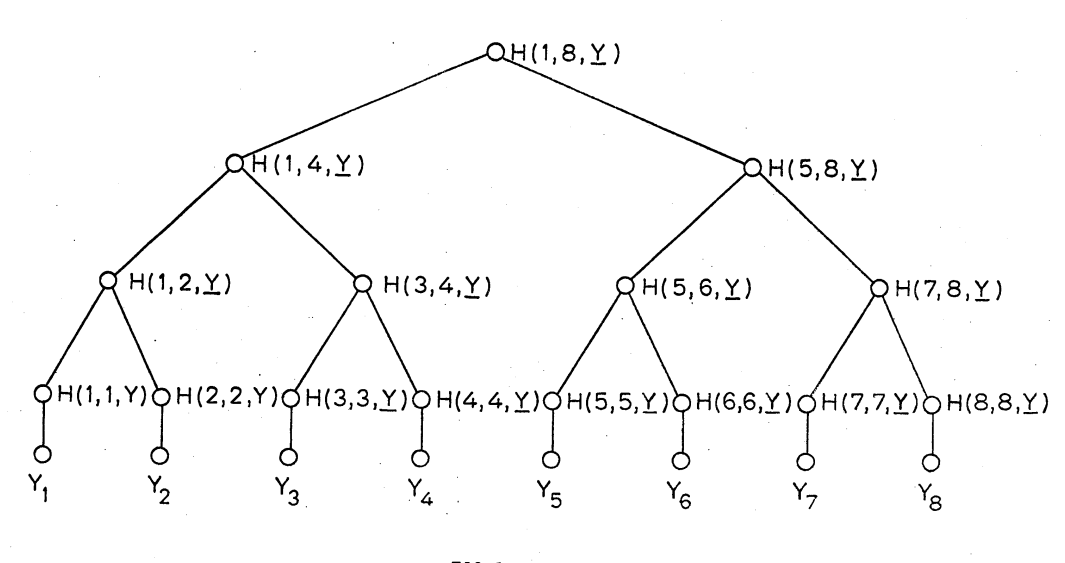
\includegraphics[width=0.7\linewidth]{merkle.png} \\ Рис. 1. Пример дерева Меркле при $n = 3$}
\end{figure}

\begin{figure}[h!]
\center{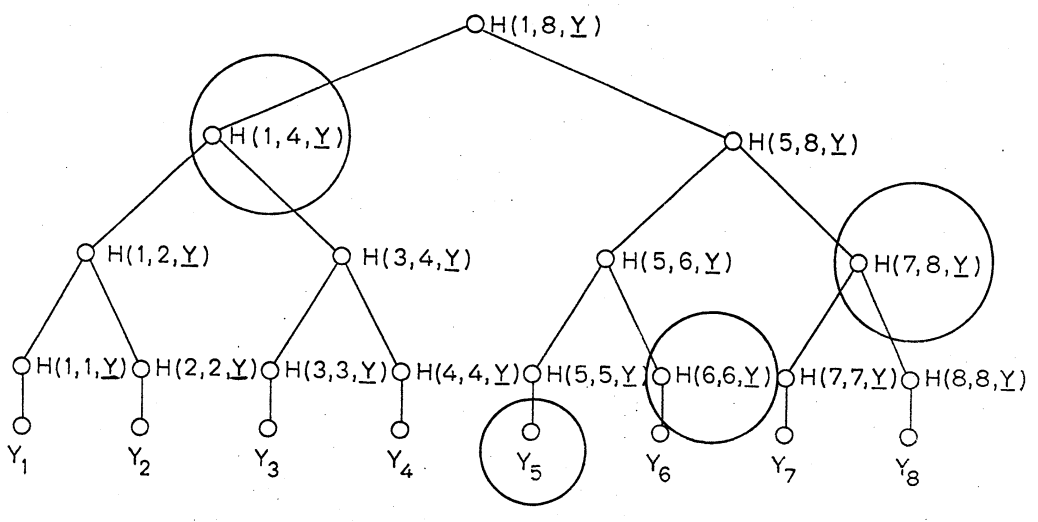
\includegraphics[width=0.7\linewidth]{image.png} \\ Рис. 2. Путь подписания в дереве Меркле при $n = 3$}
\end{figure}

\subsubsection{Анализ схемы подписи Меркля-Лампорта}

В работе \cite{lamport1} рассматриваются возможности проведения злоумышленником следующих атак: 

\begin{enumerate}
    \item Злоумышленник может полностью вычислить секретный ключ (FB);
    \item Злоумышленник может подделать подпись для любого сообщения (UU);
    \item Злоумышленник может подделать подпись для некоторых сообщений по своему выбору (SU);
    \item Злоумышленник может подделать подпись для одного произвольного сообщения (EU).
\end{enumerate}

При этом рассматриваются злоумышленники со следующими возможностями:

\begin{enumerate}
    \item Злоумышленник может изучать только открытый ключ и цифровые подписи набора случайных сообщений (RMA);
    \item Злоумышленник может изучать только открытый ключ и цифровые подписи набора выбранных им сообщений (CMA).
\end{enumerate}

Для введенных атак и моделей злоумышленников были получены следующие оценки сложности проведения атак и вероятности успеха (далее через $m$ обозначена длина входного сообщения $M$, используемого для выбора элементов секретного ключа):

\begin{enumerate}
    \item Атака EU-CMA --- сложность $O((\frac{4}{3})^\frac{m}{3})$ --- вероятность $\frac{1}{2}$;
    \item Атака SU-CMA --- сложность $O((\frac{4}{3})^\frac{m}{3})$ --- вероятность $\frac{1}{2}$;
    \item Атака UU-CMA --- сложность $O(2^{\frac{m}{2}})$ --- вероятность $\frac{1}{2}$;
    \item Атака FB-CMA --- сложность $O(2^{\frac{m}{2}})$ --- вероятность $\frac{1}{2}$;
    \item Атака EU-RMA --- сложность $O((\frac{4}{3})^m)$ --- вероятность $\frac{1}{2}$;
    \item Атака SU-RMA --- вероятность $(\frac{3}{4})^m$;
    \item Атака UU-RMA --- вероятность $(\frac{3}{4})^m$;
    \item Атака FB-RMA --- вероятность $(\frac{1}{2})^\frac{m}{2}$;
\end{enumerate}

В работе \cite{merkle1} авторами было показано, что схему подписи Меркла практически невозможно подделать при атаке с использованием выбора сообщений (CMA). В работе отмечается, что стойкость самой схемы основывается на использовании хэш-функция, стойкой к коллизиям. Также с использованием хэш-функции RIPEMD-160 на основе одноразовой подписи Лампорта была построена схема подписи, которая является безопасной относительно вычислений с использованием квантовых компьютеров.

В работе \cite{merkle2} была представлена реализацию схемы подписи Меркля на 8-битном микропроцессоре смарт-карты. Реализация предназначена для 8-битных микроконтроллеров AVR, семейства 8-битных RISC-микроконтроллеров. Для реализованной схемы подписи было получено, что время создания подписи быстрее, чем у RSA, и сравнимо с ECDSA.


Как отмечается в работе \cite{lamport} схема подписи Лампорта не самая практичная схема цифровой электронной подписи, так как для каждого сообщения приходится генерировать новую пару ключей. При этом также отмечается, что неизвестно никаких алгоритмов с полиномиальным временем, которые могли бы подделать фальшивую подпись алгоритма Лампорта со сколь угодно значимой вероятностью, даже при использовании квантового компьютера и квантовых вычислений.

\subsection{Схема подписи CFS(Courtois, Finiasz, Sendrier)}

Описание данной схемы подписи приводится на основе оригинальной статьи \cite{cfs} разработчиков данной схемы.

В схеме подписи используются следующие параметры:

\begin{enumerate}
    \item Целые числа $n$ и $k$, являющиеся параметрами безопасности;
    \item $n$-мерные битовые векторы $z, s, s_i$, где $i = 0, 1, 2, ...$;
    \item Хэш-функция $h$, выдающая $n-k$ бит на выходе;
    \item Случайная невырожденная битовая матрица $S$ из $(n - k)$ строк и $(n - k)$ столбцов;
    \item Случайная перестановочная битовая матрица $P$ из $n$ строк и $n$ столбцов;
    \item Секретный ключ $H_0$ --- битовая матрица из $(n-k)$ строк и $n$ столбцов;
    \item Открытый ключ $H = S \cdot H_0 \cdot P$;
\end{enumerate}

Генерация подписи для сообщения $M$ происходит по следующему алгоритму:

\begin{enumerate}
    \item С использованием хэш-функции $H$ вычисляется значение $s = h(M)$;
    \item Вычисляются значения $s_i = h(s \mathbin\Vert i)$ для каждого $i = 0, 1, 2, ...$;
    \item Необходимо найти значение $i_0$ --- наименьшее значение $i$ такое, что $s_i$ можно декодировать;
    \item Декодировать $s_i$ --- то есть найти такое $z$, что $H \cdot z^{T} = s_{i_0}$;
    \item Для вектора $z$ необходимо вычислить его индекс $I_z$: $I_z = 1 + \binom{i_1}{1} + ... \binom{i_t}{t}$, где $i_1 < ... < i_t$ --- позиции ненулевых битов в $z$ (стоит отметить, что данное преобразование выполняется для уменьшения длины подписи);
    \item Подписью сообщения $M$ является пара $(I_z, i_0)$.
\end{enumerate}

Проверка подписи $(I_z, i_0)$ для сообщения $M$ происходит по следующему алгоритму:

\begin{enumerate}
    \item Необходимо восстановить по индексу $I_z$ значение $z$;
    \item Вычисляется значение $s_1 = H \cdot z^{T}$;
    \item Вычисляется значение $s_2 = h(h(M) \mathbin\Vert i_0)$;
    \item Подпись считается верной, если $s_1 = s_2$.
\end{enumerate}


\subsection{CRYSTALS–Dilithium}

Описание схемы электронной подписи CRYSTALS–Dilithium приводится на основе работы \cite{crystals} авторов данной схемы.

В алгоритмах схемы подписи CRYSTALS–Dilithium в зависимости от необходимого уровня стойкости могут использоваться следующие наборы параметров: 

\begin{figure}[h!]
\center{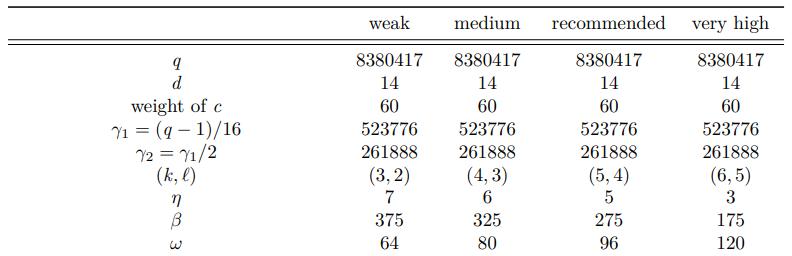
\includegraphics[width=0.7\linewidth]{crystals.png} \\ Рис. 3. Наборы параметров CRYSTALS–Dilithium}
\end{figure}

Опишем алгоритм генерации ключевой пары:

\begin{enumerate}
    \item Выбираются 256-битные значения $\rho$ и $K$;
    \item Выбираются случайные векторы $s_1$ и $s_2$ размеров $l$ и $k$ соответственно; элементами векторов являются многочлены из кольца $R_q = \mathbb{Z}_q[x]/(x^n + 1)$ с коэффициентами не больше $\eta$;
    \item С использованием значения $\rho$ по некоторому алгоритму строится матрица $A$ из $k$ строк и $l$ столбцов с элементами из $R_q$;
    \item Вычисляется вектор $t = (t_1, t_0) = As_1 + s_2$;
    \item Вычисляется 384-битный вектор $tr = CRH(\rho \mathbin\Vert t_1)$, где $CRH$ --- некоторая устойчивая к коллизиям хэш-функция;
    \item Публичным ключом является пара $(\rho, t_1)$;
    \item Секретным ключом является шестерка $(\rho, K, tr, s_1, s_2, t_0)$.
\end{enumerate}

Генерация подписи для сообщения $M$ происходит по следующему алгоритму:

\begin{enumerate}
    \item С использованием значения $\rho$ по некоторому алгоритму строится матрица $A$ из $k$ строк и $l$ столбцов с элементами из $R_q$;
    \item Вычисляется 386-битное значение $\mu = CRH(tr \mathbin\Vert M)$;
    \item С использованием значений $K, \mu, \kappa$  ($\kappa$ --- итерационный коэффициент) вычисляется $l$-мерный вектор $y$, состоящий из многочленов из кольца $R_q$ с коэффициентами не больше $\eta$;
    \item Вычисляется значение $Ay$, старшие биты сохраняются в $w_1$;
    \item С использованием $w_1$ и $\mu$ создается многочлен $c$ из кольца $R_q$, имеющий ровно 60 ненулевых коэффициентов, которые равны 1 или -1; данное преобразование реализуется открытой функцией $H = H(\mu \mathbin\Vert w_1)$;
    \item Вычисляется значение $z = y + cs_1$, являющееся потенциальной подписью;
    \item Выделяются младшие биты выражения $Ay - cs_2$ и сохраняются в $r_0$;
    \item Анализируются коэффициенты в $z$ и $r_0$: если коэффициенты не удовлетворяют определяемым параметрами схемы значениям, то необходимо перейти на новую итерацию к шагу 3;
    \item Создается подсказка $h$для подписи $z$; анализируются коэффициенты в $ct_0$ и число единиц в $h$: если коэффициенты и число единиц не удовлетворяют определяемым параметрами схемы значениям, то необходимо перейти на новую итерацию к шагу 3;
    \item Подписью сообщения $M$ считается набор значений $\sigma = (z, h, c)$.
\end{enumerate}

Проверка подписи $\sigma = (z, h, c)$ для сообщения $M$ происходит по следующему алгоритму:

\begin{enumerate}
    \item С использованием значения $\rho$ по некоторому алгоритму строится матрица $A$ из $k$ строк и $l$ столбцов с элементами из $R_q$;
    \item Вычисляется 386-битное значение $\mu = CRH(CRH(\rho\mathbin\Vert t_1)\mathbin\Vert M)$;
    \item С использованием подсказки $h$ определяется значение $w_1'$;
    \item Подпись считается верной, если:
    \begin{itemize}
        \item все коэффициенты $z$ меньше, чем $\gamma_1 - \beta$;
        \item $c = H(\mu \mathbin\Vert w_1')$;
        \item число единиц в векторе-подсказке $h$ не больше, чем $w$.
    \end{itemize}
\end{enumerate}

Подробная схема подписи CRYSTALS–Dilithium приведена на Рисунке 4.

\begin{figure}[h!]
\center{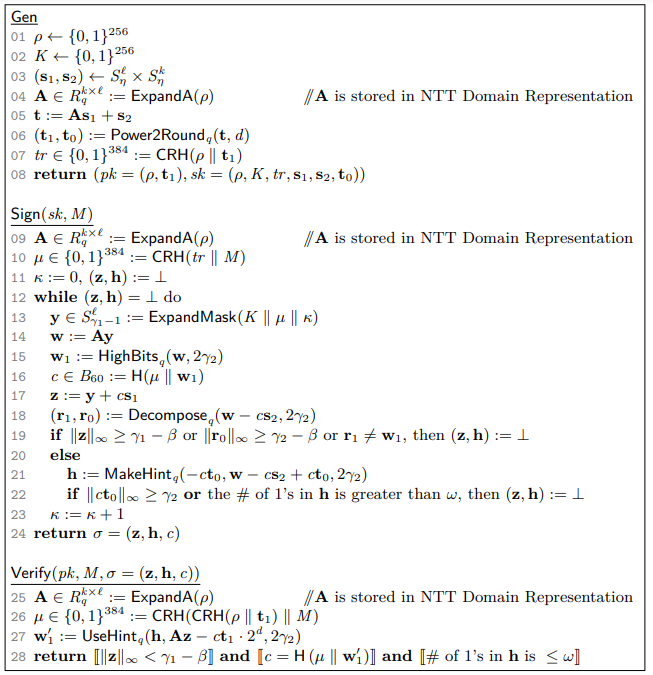
\includegraphics[width=0.7\linewidth]{dil.png} \\ Рис. 4. Схема алгоритма CRYSTALS–Dilithium}
\end{figure}

\section{Заключение}

В работе были описаны основные архитектуры, используемые при построении цифровых подписей: конструкция Hash-and-Sign и преобразование Фиата-Шамира, а также были рассмотрены следующие схемы цифровых подписей: DSA, ECDSA, ГОСТ Р 34.10-1994, ГОСТ 34.10-2018, схема подписи Фиата-Шамира, схема подписи Шнорра, схема подписи CFS (Courtois, Finiasz, Sendrier), подпись CRYSTALS–Dilithium. Также более подробно была рассмотрена схема цифровой подписи Меркля-Лампорта. Схема подписи Меркля-Лампорта может считаться одной из самых стойких и безопасных криптографических схем цифровой подписи: данная схема является устойчивой как к классическим атакам, так и к атакам с использованием квантовых вычислений, а, в частности, стойкость самой схемы основывается на использовании хэш-функция, стойкой к коллизиям.

\end{document}